\subsection{State of the Art}
% Review all of the current experimental evidence pertaining to my area of research
\todo[inline]{Talk quantum electron spin, projective measurement vs non-projective measurement (bloch sphere), about technology behind SETs}
\subsubsection{Quantum Information}
\todo[inline]{Fix this, too much detail on spin}
\todo[inline]{Talk about state space of qubits vs classical bits}
A quantum computer is composed of quantum bits of information, known as qubits. The difference between a classical bit and a quantum bit is the concept of quantum entanglement. Where any classical bit can be read and written independently of other bits in the system, the same cannot always be said of quantum bits. Reading or writing to a qubit can cause other entangled qubits in the system to change, as a single qubit no longer has a defined binary state, but it can be in a superposition of a logical "1" or "0" state. This superposition increases the information density of a quantum system, and to represent a fully entangled n-qubit system in a classical computer requires $2^n$ bits. \cite{bennett2000quantum}

In the devices manufactured by \gls{cqc2t} qubit is created from the physical property of an electron known as spin. Spin is the intrinsic magnetic moment of nano structures, essentially a small magnetic dipole, that can point in any direction in free space. For an electron, you can measure the value of this magnetic moment to be $S = \frac{\hbar}{2}$ (denoted "spin one half"). Despite this freedom of orientation, if you were to measure this spin in an arbitrary orientation, you will always find the spin to be aligned or anti-aligned to the axis of measurement (with some exceptions). For example, if you were to measure in the z-axis you would find the following:
$$S_x = 0; S_y = 0; S_z = \pm\frac{\hbar}{2}$$

Where the sign indicates alignment or anti-alignment.
However, if you were to then measure shortly after on the x-axis you would find that the spin has become indistinguishable.

that can only be observed in one of two possible states at a time. These states are named "spin-up" or "spin-down", which corresponds to the north pole pointing up or down, respectively, with regards to the axis of measurement (typically the vertical z-axis). 
\label{zeeman}
If you apply an external magnetic field to these spins, you introduce an energy difference between the spin-up and spin-down states, known as the Zeeman splitting. Using this energy difference, we can perform a spin-dependent readout from a special device, introduced in the next section.
%\subsubsection{}
\todo[inline]{Talk about the electron spin here}
\subsubsection{Quantum Devices}
\todo[inline]{Talk about the SET here}
A quantum device is any device that operates on the principles of quantum mechanics. An example is a \gls{set}, where the simplest variety can be described using the equivalent electrical circuit \cite{devoret2000amplifying} shown in Figure \ref{fig::set_circuit}. The components between the source and drain are called tunnel junctions, which can allow electrons to travel through them, even if the energy of the barrier is higher than the energy of the electron. Due to the arrangement of these components, an island is formed between each node of the typical FET transistor, which is coupled to the gate capacitively and to the drain and source through the tunnel junctions, but it is otherwise electrically isolated from the rest of the system.

Due to the isolation of the island, the only way for it to gain or lose a charge is through the drain or source. However, due to the capacitive coupling to the gate through $C_G$, energy is required to increase the charge of the island (assuming $V_G$ is constant), and as the energy of the island is given by $$E_C = \frac{Q^2}{2 C_\Sigma} ; C_\Sigma = C_D + C_S + C_G$$, we can define a quantity known as the charging energy of the capacitor. Adding or removing a single electron from the island would require an energy $\Delta E = \frac{e^2}{2 C}$ which can be on the order of 1 meV. This energy describes the difference in potential created by moving an electron from infinitely far away to on the island, though much smaller charge differences are realisable, and a charge-continuum is formed when the dielectric charge is accounted for.

Figure \ref{coulomb_blockade}, shows the relationship between the potential energy of the island and conductance through the drain-source. The upper diagram shows all lower energy states are filled, and thus no electron can pass from the source to the island. If we then raise the island potential up, akin to lowering the gate voltage (we assume at this point that the gate capacitor does not discharge), we have created an allowable energy level that can be filled from the source, and can then later tunnel to the drain. While the electron is on the island, there are no further available energy states and thus, we have created a transistor which will only allow a single electron to pass from source to drain at a time.

\begin{figure}[htbp!]
	\centering
	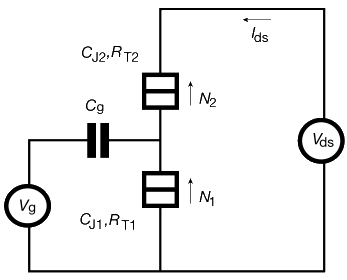
\includegraphics[width=0.6\textwidth]{set_circuit}
	\caption{Equivalent electrical circuit of an \gls{set}}
	\label{fig::set_circuit}
\end{figure}

\begin{figure}[htbp!]
	\centering
	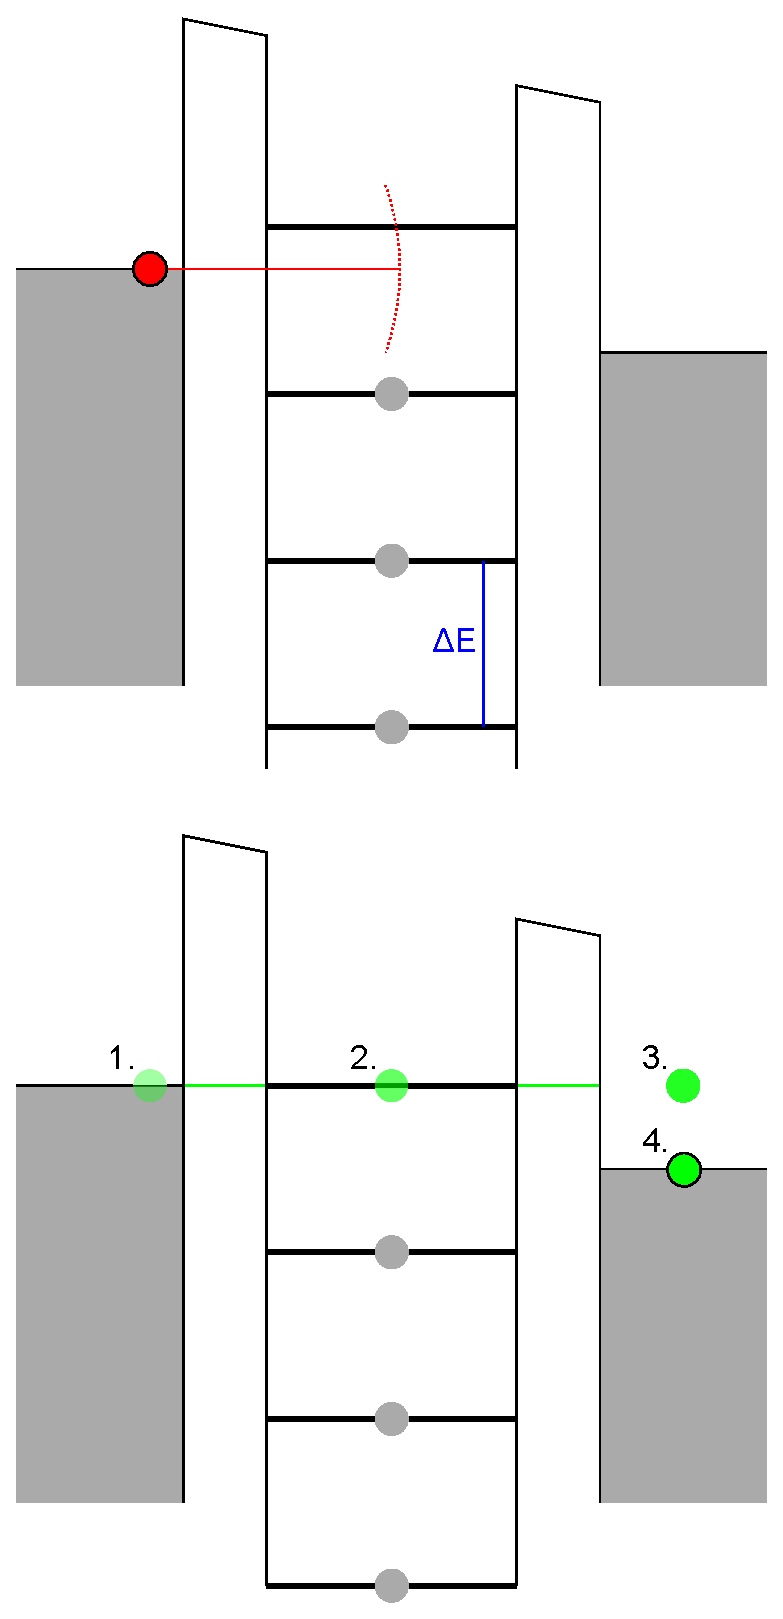
\includegraphics[width=0.6\textwidth, height=0.8\textheight]{coulomb_blockade}
	\caption{A Coulomb Blockade \cite{coulomb_blockade} forms due to electrostatic potential difference between island and source.\\ In the upper diagram, all allowable energy states are below the Fermi energy of the reservoir, hence no transmission can occur.\\ In the lower diagram, the potential of the quantum well has been raised, and now an empty state can be occupied by an electron from the source, which will subsequently tunnel off to the drain.}
	\label{coulomb_blockade}
\end{figure}

\begin{figure}[htbp!]
	\centering
	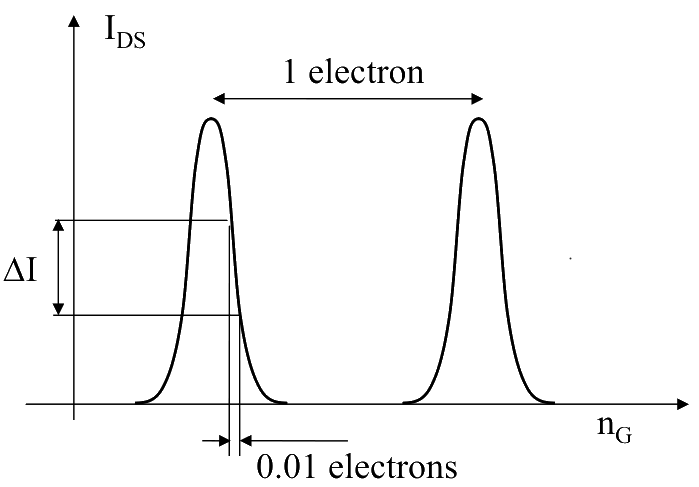
\includegraphics[width=0.8\textwidth]{coulomb_peaks}
	\caption{Coulomb Peaks form due to the discrete energy levels allowed on the island}
	\label{fig::coulomb_peaks}
\end{figure}


\todo[inline]{Talk about spin dependent tunnelling}

Recalling the Zeeman splitting energy (Section \ref{zeeman}) that is created through the application of an external magnetic field, if we can then shift the average energy level, we can allow the higher energy state to be transmitted through the coulomb blockade, while the lower energy state will not be transmitted, due to the coulomb blockade. This is known as spin-dependent tunneling, and in silicon, the higher energy state is spin up.

\begin{figure}[htbp!]
	\centering
	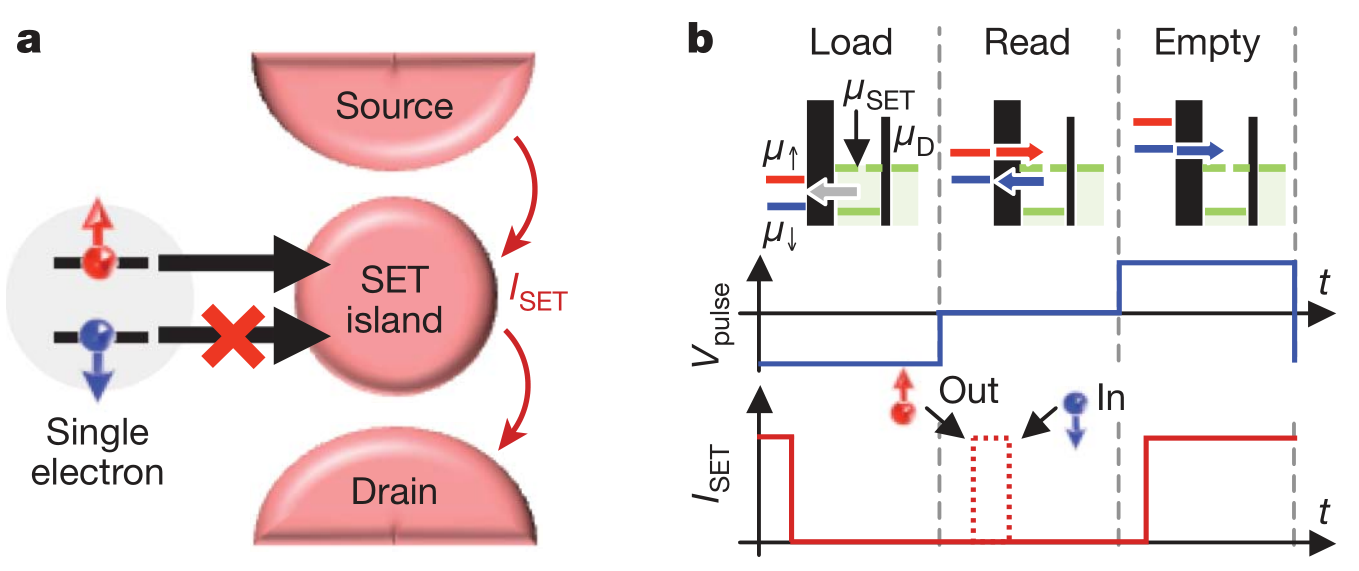
\includegraphics[width=\textwidth]{set_loading}
	\caption{The initialisation procedure of an \gls{set}}
	\label{fig::set_loading}
\end{figure}

\begin{figure}[htbp!]
	\centering
	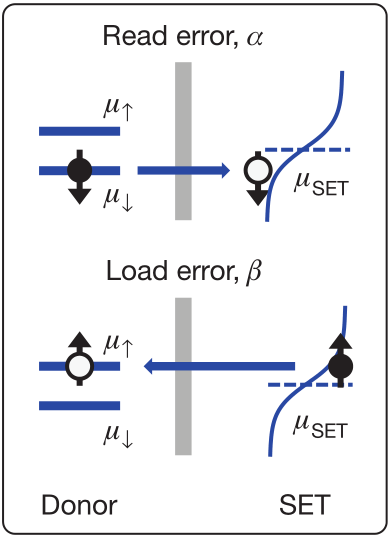
\includegraphics[height=0.5\textheight]{readout_errors}
	\caption{Load and read errors that occur when the \gls{set} is in the readout position}
	\label{fig::errors}
\end{figure}


\todo[inline]{Talk about the place of digital feedback in quantum systems}
\todo[inline]{find more digital feedback stuff}
Digital feedback has recently been explored in the development of a quantum computer. For example, it has been used to reduce error in resonance estimation \cite{bonato2015optimized} and increase coherence time of a single qubit through adjusting control parameters \cite{shulman2014suppressing}.